\begin{figure*}[t] 
  \centering
  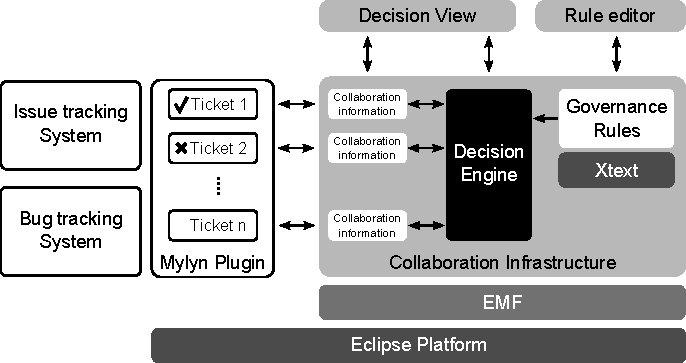
\includegraphics[width=0.65\textwidth]{./figures/architecture}
  \caption{Architecture of the developed tool.}
  \label{fig:architecture}
\end{figure*}


Our approach has been implemented as an Eclipse plug-in \footnote{The prototype can be downloaded from https://code.google.com/a/ eclipselabs.org/p/governance-rules-mylyn/} providing a collaborative infrastructure allowing developers and project managers to define and apply governance rules. 

Figure \ref{fig:architecture} summarizes the architecture of our prototype tool. We rely on Mylyn\footnote{http://www.eclipse.org/mylyn} for accessing and updating the tasks of the development project we are collaborating on. Mylyn incoporates several connectors covering a great variety of tracking systems\footnote{The complete list of supported tools can be found at http://wiki.eclipse.org/index.php/Mylyn\_Extensions}. The collaboration models storing all the information about the ongoing discussions, votes, etc. are implemented on top the EMF \footnote{http://www.eclipse.org/emf} Eclipse component. 

Our DSL to define governance rules has been developed in Xtext\footnote{http://www.eclipse.org/Xtext}, a tool to create textual DSLs in Eclipse. In Xtext, DSLs are described by an annotated grammar from which the required tooling is generated (e.g., specific editor, syntax highlighting, auto-completion, content assistance, etc.). We defined the grammar for our DSL and generated the corresponding DSL tooling. The plugin therefore provides a specific editor to define governance rules (see \emph{Rule editor}). 

Once the rules are defined, the collaboration information is collected in a dedicated view (see \emph{Decision View}) and, via Mylyn, linked to the project tasks as metadata. The rules plus this information are then interpreted by an engine developed in Java (see \emph{Decision Engine}) that updates the tasks status according to the governance rules defined.

Figure \ref{fig:snapshot} shows a snapshot of the platform including both the \emph{Decision view} (on the left bottom part) and the \emph{Rules editor} (on the right top part) for the Apache example presented before. Five tasks from the Apache repository (project \texttt{apache-httpd-2}) have been selected for the sake of conciseness. As can be seen, these tasks are shown in the \emph{Task List} view provided by Mylyn and in the \emph{Decision view} provided by our tool, which allows users to vote for/against these tasks. The view also includes buttons to configure the strategy (opening the \emph{Rule editor} shown in the Figure), to apply it, to login and to refresh the view. As an example, the rules have been triggered using sample votes, thus resulting in the acceptance of the first two tasks and rejection of the rest. 

\begin{figure*}[t] 
  \centering
  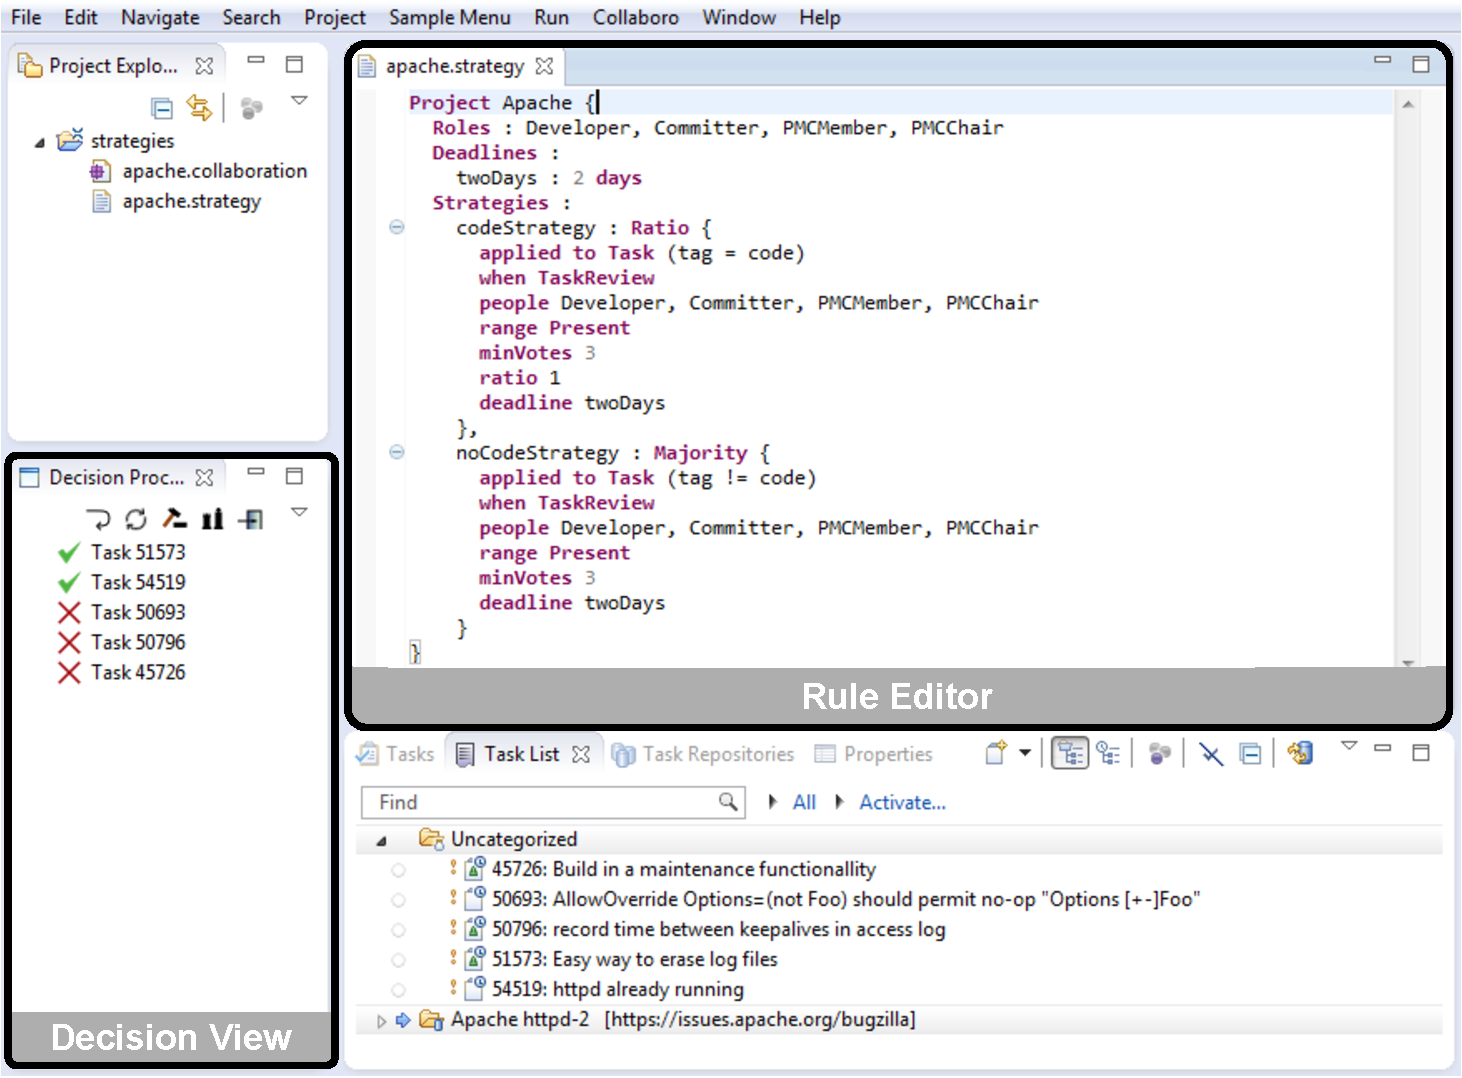
\includegraphics[width=0.85\textwidth]{./figures/snapshot}
  \caption{Snapshot of the developed tool.}
  \label{fig:snapshot}
\end{figure*}

